\newpage
\pagestyle{empty}
% If you do want an image in the colophon:
\begin{figure}
  \vspace{50pt}
  \centering
  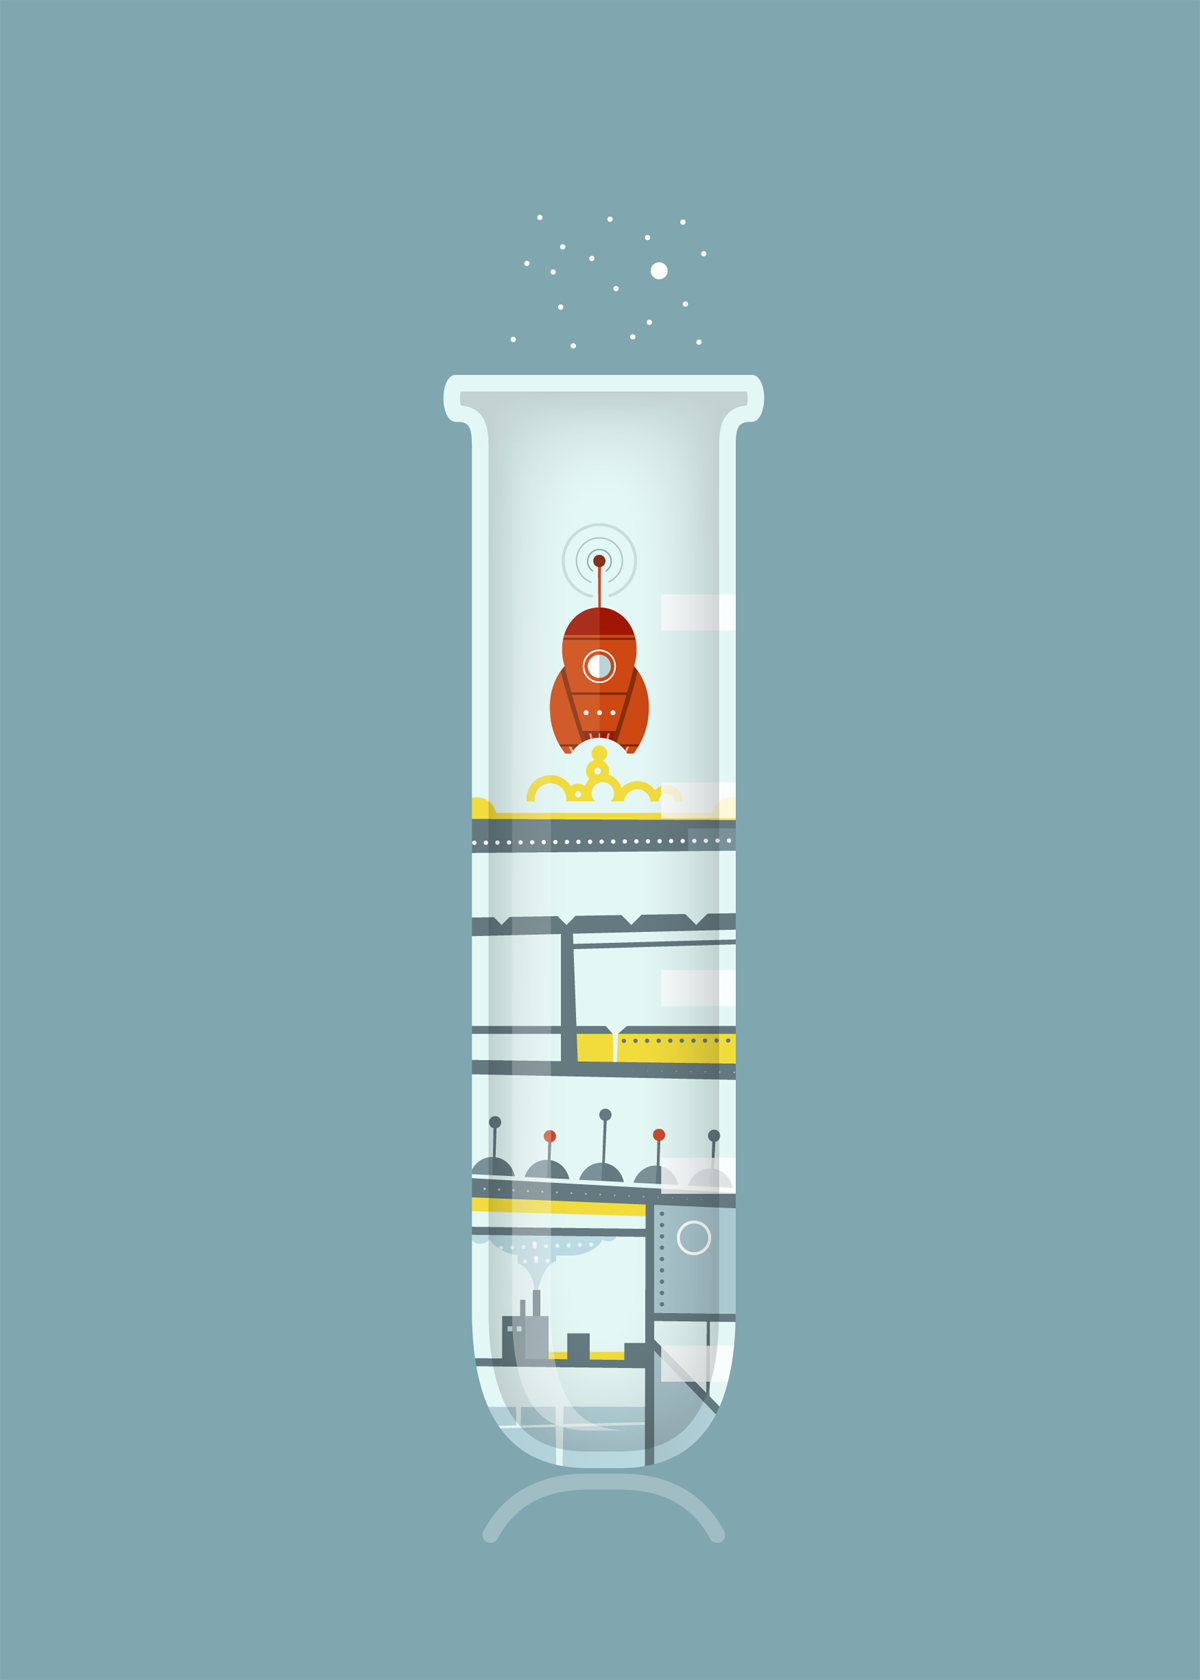
\includegraphics[width=0.51\textwidth]{./figures/colophon}
\end{figure}

% If you don't want an image in the colophon:
% \vspace*{200pt}

\begin{center}
\parbox{200pt}{\lettrine[lines=3,slope=-2pt,nindent=-4pt]{\textcolor{uni-color}{T}}{his coursework was typeset} using LaTeX, originally developed by Leslie Lamport and based on Donald Knuth's TeX. The body text is set in 12 point kpfonts, a revival of URW Palladio typeface. The above illustration, ``Science Experiment 02'', was created by Ben Schlitter and released under \href{http://creativecommons.org/licenses/by-nc-nd/3.0/}{\textsc{cc by-nc-nd 3.0}}. A template that can be used to format coursework with this look and feel has been released under the permissive \href{http://creativecommons.org/licenses/by-nc-nd/4.0/}{\textsc{cc by-nc-nd 4.0}} license, and can be found online at \href{https://cs.overleaf.com/latex/templates/maths-coursework-template/kbyhcwmjdtpf}{https://cs.overleaf.com/latex/}.}
\end{center}